

\chapter{روش پیشنهادی}
\tikzstyle{edge_style} = [draw=black,line width=0.3,-latex']
\tikzstyle{line1} = [draw=red,line width=0.3] 
\tikzstyle{line2} = [draw=black,line width=0.3] 
\tikzstyle{operator} = [draw,shape=circle,fill=white,minimum size=1.3em] 
 \tikzstyle{phase} = [draw,shape=circle,minimum size=10pt,inner sep=0pt]
 \tikzstyle{control} = [fill,shape=circle,minimum size=12pt,inner sep=0pt]
 \tikzstyle{hadamard} = [draw,shape=rectangle,minimum size=12pt,inner sep=0pt]
\tikzstyle{line} = [draw, -latex']
\tikzstyle{cir1} = [fill=blue!20,shape=circle,minimum size=15pt,inner sep=0pt] 
\tikzstyle{cir2} = [fill=yellow,shape=circle,minimum size=15pt,inner sep=0pt]
\tikzstyle{vertexs}=[draw,minimum width=0pt,minimum height=15pt]
\tikzstyle{cir3} = [fill=green!30,shape=circle,minimum size=15pt,inner sep=0pt]
\algnewcommand\algorithmicforeach{\textbf{for each}}

\algdef{S}[FOR]{ForEach}[1]{\algorithmicforeach\ #1\ \algorithmicdo}

\newpage
‎\renewcommand{\baselinestretch}{2}\normalsize‎
\label{proposed approach}
\section{روش پيشنهادي}
 در این فصل، روش پیشنهادی برای ساخت مدار کوانتومی توزیع شده با هدف کاهش تعداد دورنوردی‌های کوانتومی ارائه خواهد شد. در ابتدا مقدمات و کلیات روش شرح داده شده و در ادامه جزئیات هر قسمت بحث خواهد گردید.
\section{مقدمه}
\label{مقدمه}
با توجه به معماری ارائه شده در فصل پیشین، در این رساله برآنیم تا با تمرکز بر لایه دوم، یک مدار کوانتومی از سطح اول دریافت نموده، و بتوانیم آن را بین سیستم‌های کوانتومی به طور مناسب با در نظرگرفتن تعدادی هدف توزیع نماییم. همانطور که در معماری سیستم‌های توزیع شده بیان شد، این مساله از وظایف لایه‌ي دوم می‌باشد. در طراحی این لایه، با چند مساله‌ي اصلی و چالش مواجه هستیم که عبارت‌اند از:
%\begin{figure}[t!]
%\begin{center}
%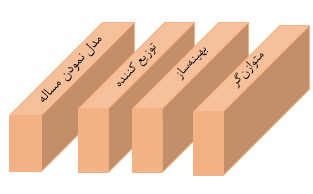
\includegraphics[scale=0.7]{level2.jpg}
%\caption{نیازمندی‌های اصلی در لایه دوم شکل \ref{distribute} }
%\label{level2}
%\end{center}
%\end{figure}
\begin{itemize}
\item
\textbf{ارائه‌ی مدلی مناسب}:
جهت بررسی و طراحی این سیستم، در ابتدا بایستی بتوان آن را به طور دقیق مدل‌سازی نمود و مساله با استفاده از متغیرها و روابط ریاضی توصیف شود. در سطح اول الگوريتم پيشنهادي به مدل‌سازی دقیقي از مساله با استفاده از برنامه ریزی خطی پرداخته شده است.
\item
\textbf{ افرازبند\footnote{\lr{Partitionner}} یا توزیع کننده}:
پس از مدل‌سازی رياضي، یکی از مهمترین مسائلی که طراحی سیستم‌های کوانتومی توزیع شده با آن مواجه است، استفاده از الگوریتم‌های افرازبندی جهت توزيع كيوبيت‌هاي مدار است. بنابراین یافتن یک الگوریتم جهت افرازبندی مدار امری ضروری است. 
\item
\textbf{بهینه‌ساز\footnote{\lr{Optimizer}}}:
همانطور که پیش‌تر اشاره شد، از آنجایی‌که تعامل کیوبیت‌ها در محیط با خطا و نویز مواجه است و عملگرهای از راه دور نسبت به عملگرهای محلی بیشتر با این خطاها مواجه هستند، پروتکل دورنوردی عملی هزینه‌بر در سیستم‌های کوانتومی است. بنابراین کاهش تعداد آن امری ضروری است. بنابراین در طراحی این سیستم نیازمند استفاده از الگوریتم بهینه سازی بوده تا بتوان تعداد مورد نظر را بهینه نمود.%یک هدف که کیوبیت‌ها بطور متعادل \lr{\footnote{Balance}} توزیع شده و تعداد دورنوردی‌های مورد استفاده  جهت ساخت این سیستم حداقل ممکن گردد. بهینه سازی تعداد دورنوردی‌ها در دوسطح انجام میگردد. در سطح اول با ارائه الگوریتمی مدار کوانتومی به $K$ افراز با هدف کاهش تعداد دورنوردی‌ها و توزیع  متعادل کیوبیت‌ها توزیع می‌گردد و در سطح دوم با ارائه‌ی تعدادی قانون این سیستم بهینه‌تر می‌گردد.
\item
\textbf{متوازن‌کننده\footnote{\lr{Load Balancer}}}:
گاهی اوقات کاهش بیش از اندازه‌ی تعداد پروتکل دورنوردی منجر به عدم توازن در تعداد کیوبیت‌های هر زیر سیستم می‌گردد و از آن‌جایی که هر سیستم‌های کوانتومی در تعداد کیوبیت‌ها دچار محدودیت هستند، بنابراین همزمان با کاهش تعداد دورنوردی‌های کوانتومی، توزیع متوازن کیوبیت‌ها نیز هدف اصلی قرار می‌گیرد. بنابراین از دیگر مسائلی که در طراحی سیستم‌های کوانتومی توزیع شده با آن مواجه هستیم، مساله توزیع متوازن بار یا همان تعداد کیوبیت‌ها است. 
\end{itemize}

به دليل پيچيدگي بالاي سيستم‌هاي كوانتومي، طراحي سيستم‌هاي كوانتومي توزيع شده و بهينه‌سازي آن در يك سطح امري دشوار است. راه‌کار پیشنهادی در این رساله این است تا بتوان سیستم مورد نظر را در دو سطح ّه طور سلسله مراتبی بهینه نمود. این دو سطح عبارت‌اند:
\begin{itemize}
\item

 سطح اول: در این سطح در ابتدا مدلی ریاضی از  مساله‌ی افرازبندی مدار کوانتومی ارائه خواهد شد. سپس با تبدیل مدار کوانتومی به یک گراف تعداد برش کمینه جهت افرازبندی این مدار به $K$ زیر سیستم بدست خواهد آمد. تعداد برش‌های بدست آمده همان تعداد دروازه‌های سراسری بین سیستم‌ها خواهد بود. در این سطح، زمانبندی اجرای دروازه‌های کوانتومی در نظر گرفته نمی‌شود. خروجي اين سطح برچسب‌گذاري كيوبيت‌ها برحسب شماره افرازي است كه در آن قرار مي‌گيرند.


\item
 سطح دوم: با توجه به افرازبندی بدست آمده از سطح اول، در مرحله‌ی اجرای دروازه‌های سراسری کوانتومی، زمانی که یکی از کیوبیت‌های این دروازه از مبدا خود به مقصد مورد نظر دورنورد می‌گردد، ممکن است کیوبیت دورنورد شده بتواند توسط تعدادی دروازه سراسری دیگر با رعایت محدودیت‌های پیش نیازی مورد استفاده قرار گرفته و در نتیجه موجب کاهش تعداد دورنوردی‌ها گردد. در این سطح به سوالات زیر پاسخ داده می‌شود: 
\begin{itemize}
\item
زمانی‌که یک کیوبیت از مبدا خود به مقصد دورنورد می‌شود، چه‌زمانی به مقصد خود بازگردد؟ گاهی اوقات با دورنورد شدن یک کیوبیت می‌توان چند دروازه را همزمان اجرا نمود به شرطی که محدودیت‌های پیش نیازی آن‌ها رعایت شده باشند.
\item
در یک دروازه‌ی سراسری دو کیوبیتی، کدام کیوبیت این دروازه دورنورد شود؟  تعداد دروازه‌های سراسری که با دورنورد نمودن کیوبیت کنترلی یا هدف می‌توانند اجرا شوند، در بیشتر موارد متفاوت بوده و در نتیجه پاسخگویی به این سوال امری مهم محسوب می‌گردد.
\end{itemize}
\end{itemize}
در ادامه در ابتدا به بیان نمادها و تعاریف مورد استفاده، سپس به توضیح و پیاده‌سازی روش‌های پیشنهادی پرداخته شده است.

\section{تعریف‌ها و نمادها}
\subsection{متغیرهای مورد استفاده}
مجموعه متغیرهای استفاده شده در این رساله در جدول \ref{notation} آورده شده است.
\begin{table}[h]
\centering
\caption{\small{متغیرهای مورد استفاده در مدل ریاضی }}
\label{notation}
\footnotesize\rm
\begin{tabular}{cc}
\hline
متغیر&توصیف\\
\hline
$N_{g}$&تعداد دروازه‌ها\\
$N_{q}$&تعداد کیوبیت‌ها\\
$run_{i}$&حالت اجرای دروازه‌ی \lr{i}\\
$P_{i}$&شماره افرازی که کیوبیت \lr{i} در آن قرار دارد\\
$N_{t}$&تعداد دورنوردی‌ها\\
$K$&تعداد افرازها\\
$\omega$&نرخ عدم تعادل \\
$N_{non}$&تعداد دروازه‌های سراسری\\
$N_{2qubit}$&تعداد دروازه‌های دوکیوبیتی\\
\hline
\end{tabular}
\end{table}
\subsection{انواع دروازه‌ها در مدل پیشنهادی}
مجموعه دروازه‌های مورد استفاده در مدل پیشنهادی به صورت زیر در نظر گرفته شده است:
\begin{itemize}
\item
\textbf{دروازه‌ی تک کیوبیتی:}
این دروازه یک دروازه‌ی محلی به شمار می‌آید و به صورت زیر نشان داده می‌شود:
\begin{equation}
g\_name(q_{i},P_{i})
\label{eq23}
\end{equation}
بطوری که $q_{i}$ بیانگر شماره کیوبیتی است که دروازه‌ی تک کیوبیتی روی آن عمل نموده و $P_{i}$ بیانگر شماره افرازی است که کیوبیت $q_{i}$ در آن قرار دارد.

\item
\textbf{دروازه‌ی محلی\footnote{\lr{Local gate}}: }
 دروازه‌ای است که کیوبیت هدف و کنترلی آن در یک افراز قرار داشته باشند و به صورت زیر نشان داده می‌شود:
\begin{equation}
g\_name(q_{t},q_{c},P_{t})
\label{eq24}
\end{equation}
عبارت بالا بیانگر این است که این دروازه‌ی محلی دارای کیوبیت کنترلی $q_{t}$ و کیوبیت هدف $q_{c}$ بوده و این دروازه در افراز $P_{t}$ قرار دارد. 

\item
\textbf{دروازه‌ی سراسری \footnote{\lr{Global gate}}: }
دروازه‌ای است که کیوبیت هدف و کنترلی آن در دو افراز متفاوت قرار دارند. یک دروازه‌ی سراسری به صورت زیر نشان داده می‌شود.
\begin{equation}
g\_name(q_{c},q_{t},P_{c},P_{t})
\label{eq25}
\end{equation}

عبارت بالا بیان می‌کند که دروازه‌ی \lr{g\_name} دارای کیوبیت هدف $q_{t}$ و کیوبیت کنترلی $q_{c}$ بوده که به ترتیب در افراز‌های $P_{t}$ و $P_{c}$ قرار دارند.
\end{itemize}
دروازه‌های تک کیوبیتی و دروازه‌های محلی برای اجرا نیاز به دورنوردی کوانتومی نداشته در حالی که دروازه‌های سراسری برای اجرا نیاز به این دارند که برای اجرا، دو کیوبیت آن در یک زیر سیستم قرار گرفته و سپس اجرا شوند. بنابراین نیاز به دورنوردی کوانتومی دارند.
\section{افرازبندی سطح اول}
هدف از این سطح این است که بتوان کیوبیت‌های مدار را در تعدادی زیر سیستم کوانتومی توزیع نمود و یک سیستم توزیع شده ایجاد نمود، به‌طوری‌ که تعداد ارتباطات بین زیرسیستم‌های کوانتومی حداقل شود. از آن‌جایی که این مساله \lr{NP-Hard} است \cite{andreevvv}، الگوریتمی دقیق با زمان جندجمله‌ای برای آن وجود ندارد. در این سطح در ابتدا به بیان مدلی ریاضی از مساله افرازبندی مدار کوانتومی پرداخته شده و سپس دو الگوریتم جهت افراز‌بندی کیوبیت‌ها ارائه می‌‌گردد. در الگوریتم اول به توزیع متوازن کیوبیت‌ها در دو زیرسیستم و در الگوریتم دوم به توزیع آن‌ها در چند افراز پرداخته شده است. 
\subsection{مدل‌سازی ریاضی }


تعریف مساله: فرض شود مدار کوانتومی\lr{QC} شامل مجموعه‌ای از دروازه‌های کوانتومی $\mathcal{G}=\{g_{j}| j \in\{1,..,N_{2qubit}\}\}$  و مجموعه‌ای از کیوبیت‌ها
 $Q=\{q_{i}| i \in\{1,...,N_q\}\}$
 باشد. جهت مدل سازي اين مساله نياز است كه مجموعه‌اي از متغيرهاي دودويي به صورت زير تعريف گردد. 
\abovedisplayskip=3pt
\belowdisplayskip=0pt
\[
p_{i,k}=
\begin{cases}
 1& \text{اگر $q_i$ در افراز $k$ قرار داشته باشد.}\\
0& \text{در غیر اینصورت}
 \end{cases}
\]


\[
f_{j}=
\begin{cases}
 1& \text{اگر دروازه‌ی $g_j$ دروازه‌ای سراسری باشد. }\\
0& \text{در غیر اینصورت}
 \end{cases}
\]


\begin{equation}
\min \sum\limits_{j=1}^{N_{2qubit}} f_{j} 
\label{eq16}
\end{equation}
\begin{equation}
\sum\limits_{i=1}^{N_{q}} p_{i,k} \leq (1+\omega)|Q| /K \quad \forall k=1,...,K
\label{eq17}
\end{equation}

\begin{equation}
\sum\limits_{k=1}^K p_{i,k}=1    \quad \forall i=1,...,N_q
\label{eq18}
\end{equation}

\begin{equation}
f_{j}\geq p_{i_2,k}-p_{i_1,k} \quad \forall k=1,...,K, \quad g_j(i_{1},i_{2}) \in\mathcal{G}
\label{eq19}
\end{equation}

\begin{equation}
f_{j}\geq p_{i_1,k}-p_{i_2,k} \quad \forall k=1,...,K, \quad g_j(i_{1},i_{2}) \in\mathcal{G}
\label{eq20}
\end{equation}

 $f_{j} \in\{0,1\}, p_{i_1,k}\in\{0,1\} \quad \forall i=1,...N_{q}, j=1,...,N_{2qubit}, k=1,...,K$

 این رابطه‌ها به ترتیب در زیر تعریف شده‌اند:
\begin{itemize}
\item
رابطه \eqref{eq16} تابع هدف را نشان می‌دهد که این تابع به‌دنبال کمینه نمودن تعداد ارتباط‌‌ها در مدار یا همان تعداد دروازه‌های سراسری است.
\item
رابطه‌ی \eqref{eq17} شرط توزیع شدن متوازن کیوبیت‌ها را نشان می‌دهد. در این رابطه مجموعه تعداد کیوبیت‌هایی که در یک افراز قرار می‌گیرد، بایستی از مقدار $(\frac{1+\omega}{K}|Q|)$ کمتر یا مساوی باشد.
\item

رابطه \eqref{eq18} بیانگر این است که هر کیوبیت تنها به یک افراز تخصیص یابد. 
\item
در رابطه‌های \eqref{eq19} و \eqref{eq20} شرط این‌که دوکیوبیت در دو افراز جدا قرار گرفته باشند و تشکیل یک دروازه‌ی سراسری را بدهند، بررسی می‌گردد.
\end{itemize}




 
\subsection{الگوریتم توزیع کیوبیت‌ها در دو افراز}
در این بخش با استفاده از الگوریتم \lr{NSGA-II} به توزیع متوازن کیوبیت‌ها در دو افراز پرداخته شده است. اهدافی که در این الگوریتم به دنبال بهینه‌سازی آن هستیم، عبارت‌اند از:
\begin{itemize}
\item
تعداد دروازه‌های سراسری در توزیع بدست آمده\lr{(GlobalNum)}: از آنجایی هدف از افرازبندی کیوبیت‌ها، کاهش تعداد دورنوردی‌های کوانتومی بوده، كمينه نمودن تعداد دروازه‌های سراسری منجر به کاهش تعداد دورنوردی‌های کوانتومی می‌گردد. 
\item
اختلاف تعداد کیوبیت‌های بدست آمده در دو افراز \lr{(QNum)}: همانطور که قبلا بیان شد، یکی از چالش‌های اساسی در این سیستم این است که توزیع کیوبیت‌ها در افرازهای متفاوت، متعادل باشد.  بنابراین هر چه اختلاف کیوبیت‌های قرار گرفته در دو افراز به صفر نزدیک باشد، نشان دهنده‌ی توزیع متوازن آن‌ها خواهد بود. بنابراین این پارامتر به عنوان هدف دوم در الگوریتم ارائه شده در نظر گرفته خواهد شد.
\end{itemize}
طول کروموزوم بکار رفته در این الگوریتم برابر $N_q+1 $ می‌باشد. در این الگوریتم پارامتری به نام خط برش \lr{(Cutline)} تعریف شده است که بیانگر محلی است که کیوبیت‌ها از یکدیگر جدا شده و در دو افراز قرار می‌گیرند. همچنین مقادیر ژن‌های کروموزوم به صورت زیر مقدار دهی شده است:
\begin{itemize}
\item
ژن اول بیانگر مکان خط برش می‌باشد. 
\item
ژن \lr{i+1} متناظر با مکان کیوبیت \lr{i}ام در توزیع بوجود آمده می‌باشد.
\end{itemize}
 
 با توجه به موارد بیان شده به تعداد \lr{Cutline} کیوبیت در افراز اول و به تعداد \lr{$N_q$-Cutline} کیوبیت در افراز دوم قرار گرفته است. برای توضیح بیشتر در ادامه به بیان مثالی پرداخته شده است. شکل \ref{fig:a} یک مدار کوانتومی با شش کیوبیت را نشان داده و نمونه‌ای از یک کروموزوم متناظر با اين مدار، در شکل \ref{chromeelahi} آورده شده است. 
 \begin{figure}
 \centering
\includegraphics[scale=0.7]{chromeelahi.jpg}
\caption{نمونه‌ای از کروموزوم مورد استفاده در الگوریتم }
\label{chromeelahi}
 \end{figure}
 در این کروموزوم مکان خط برش در محل 2 قرار گرفته و کیوبیت‌های 1 تا 6 به ترتیب در مکان‌های 3، 1، 2، 5، 6 و 4 قرار گرفته است. مدار بدست آمده در شکل \ref{fig:b} آورده شده است.
 \begin{figure}[h]
\centering     
\subfigure[مدار کوانتومی اولیه]{\label{fig:a}\includegraphics[width=130mm]{elahisample1}}
\subfigure[چگونگی توزیع کیوبیت‌ها در دوافراز با توجه به کروموزوم ارائه شده در شکل \ref{chromeelahi}]{\label{fig:b}\includegraphics[width=130mm]{elahisample2}}
\caption{چگونگی توزیع کروموزوم‌ها با استفاده از الگوریتم \lr{NSGA-II} در دو افراز}
\label{elahisample}
\end{figure}
بعد از اعمال الگوریتم \lr{NSGA-III} روی مدار مورد نظر، جواب بهینه‌ي بدست آمده همانند مدار شکل \ref{optimalelahi} است.  در جواب بهینه‌‌ی بدست آمده کیوبیت‌های $q_4 $، $q_1 $ و $q_6 $ در افراز اول و کیوبیت‌های $q_3 $، $q_2 $ و $q_5 $ در افراز دوم قرار گرفته‌اند. همچنین مقادير پارامترهای \lr{Qnum} و \lr{GlobalNum} بترتيب برابر با 0 و 4 بدست آمده است.
 \begin{figure}[h]
\centering     
\subfigure[مدار کوانتومی بدست آمده پس از اعمال الگوریتم \lr{NSGA-III}]{\label{figa}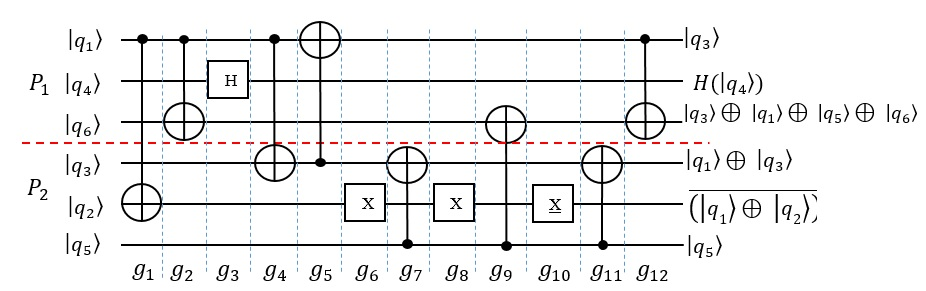
\includegraphics[width=130mm]{optimalelahi}}
\subfigure[کروموزوم بدست آمده]{\label{figb}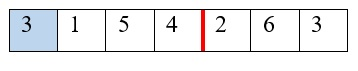
\includegraphics[width=70mm]{optimalelahich}}
\caption{جواب بهینه بدست آمده پس از اعمال الگوریتم \lr{NSGA-III} روی مدار شکل \ref{fig:a}}
\label{optimalelahi}
\end{figure}

\subsection{الگوریتم پیشنهادی جهت افرازبندی چندگانه }
از آنجایی که مساله‌ي افرازبندی کیوبیت‌ها در چند افراز \lr{NP-hard} بوده، الگوریتمی دقیق با زمان چند جمله‌ای برای آن پیشنهاد نشده است. در این قسمت به مساله افرازبندی کیوبیت‌ها در چند افراز پرداخته شده و براي حل آن  از برنامه سازی پویا استفاده گرديده است. الگوریتم 1 ساختار اصلی راه حل پیشنهادی در این مرحله را نشان می‌دهد. این الگوریتم مدار کوانتومی داده شده در ورودی مساله را با هدف کاهش تعداد دورنوردی‌های مورد نیاز با در نظر گرفتن توازن افرازها، به \lr{K} افراز توزیع نموده و از دو مرحله تشکیل شده است: در مرحله‌ی اول سعی شده است که تا بتوان مدار کوانتومی را در قالب یک گراف دو بخشی نمایش داد (خط 4 تابع \lr{QCtoBigraph}) و سپس در مرحله‌ی دوم با استفاده از برنامه سازی پویا، الگوریتمی جهت افرازبندی گراف دو بخشی ارائه گردد (خط 5 تابع \lr{DP}). خروجي اين الگوريتم تعداد دروازه‌هاي سراسري و آرايه‌ي $P$ كه بيانگر شماره افرازهايي است كه هر كيوبيت به آن تعلق گرفته است.
\begin{latin}
\begin{algorithm}
{
\fontsize{9}{1}
\caption{\lr{Main algorithm}}
\begin{algorithmic}[1]
\Function {Main} {QC, K}

\State\textcolor[rgb]{0.00,0.50,1.00}{ $\triangleright$ \lr{Input: Quantum circuit (QC), The number of partitions ($K$)}}
\State\textcolor[rgb]{0.00,0.50,1.00}{ $\triangleright$ Output: The minimum number of non-local gates, P }
\State \textcolor[rgb]{0.00,0.50,1.00}{ $\triangleright$ Step I:} G=QCtoBigraph(QC);
\State \textcolor[rgb]{0.00,0.50,1.00}{ $\triangleright$ Step II:}  $N_{non}$=DP(G,K);

\EndFunction
\end{algorithmic}
}

\end{algorithm}
\end{latin}
\begin{itemize}
\item
\textbf{مرحله‌ي اول:}
در این مرحله، مدار کوانتومی به صورت یک گراف دو بخشی نشان داده می‌شود. به طوری که مجموعه دروازه‌های مدار، در یک سمت گراف دو بخشی (بخش \lr{Y}) و در سمت دیگر آن (بخش \lr{X}) مجموعه کیوبیت‌های موجود در مدار کوانتومی قرار می‌گیرند. یال‌های اين گراف شامل دروازه‌های دو کیوبیتي مدار هستند و به صورت زیر ایجاد می‌گردند:

به ازای هر دروازه‌ی دو کیوبیتی $g_{j}(q_{c},q_{t})$، دو یال $(g_{j},q_{t})$ و $(g_{j},q_{c})$ به گراف اضافه می‌گردند. از آنجایی‌که دروازه‌های تک کیوبیتی تاثیری در افرازبندی گراف ندارند، آن‌ها در نظر گرفته نمی‌شوند. 

الگوریتم 2 چگونگی تشکیل این گراف دو بخشی را نشان می‌دهد.
\begin{latin}
 \begin{algorithm}
{
\fontsize{9}{1}
\caption{This algorithm converts quantum circuit to bigraph}
\begin{algorithmic}[2]
\Function {G=QCtoBigraph} {QC}
\State\textcolor[rgb]{0.00,0.50,1.00}{ $\triangleright$   Step I: Convert QC to Bigraph}
\State Initialize G(V,E) ,   $G.X=Q$  ,  $G.Y=\mathcal{G}$ and   $ E=\{\}$ ; \textcolor[rgb]{0.00,0.50,1.00}{ $\triangleright$ $ V=X \cup Y$}
\State\textcolor[rgb]{0.00,0.50,1.00}{ $\triangleright$  Qubits are in one part of bigraph G (part X) and gates are in other parts ( part Y)  }
   \For {each $ g_{j} \in \mathcal{G}$}
         \State $c\leftarrow$ contorol qubit of $g_{j}$;
        \State $t \leftarrow$ target qubit of $g_{j}$;
         \State  Add to $E$ edges $(c,g_{j})$ and $(t,g_{j})$;
 \EndFor
\EndFunction
\end{algorithmic}
}
\end{algorithm}
\end{latin}
در این الگوریتم در ابتدا یک گراف دوبخشی به نام \lr{G} با دو مجموعه‌ی تهی \lr{X} و \lr{Y} و بدون یال در نظر گرفته مي‌شود. سپس به ازای هر $g_j \in \mathcal{G}$ مجموعه یال‌های ذکر شده در بالا به یال‌های گراف اضافه خواهد شد. برای مثال گراف دو بخشی  مدار ارائه شده در شکل \ref{10}، در شکل \ref{11} نشان داده شده است.
\begin{figure}
\begin{center}

    \begin{tikzpicture}
    \node at (0,0) (q1) {\ket{q_{1}}};    \node at (0,-1) (q2) {\ket{q_{2}}};    \node at (0,-2) (q3) {\ket{q_{3}}};    \node at (0,-3) (q4) {\ket{q_{4}}};
    \node[control] (c20) at (2,0) {} ;edge [-] (q1);    \node[operator] (r21) at (2,-1) {} ;edge [-] (q2);    \draw[-] (2,-1.25) -- (c20);

 % Column 3
    \node[control] (c31) at (3,-1) {};    \node[operator] (r33) at (3,-2) {};    \draw[-] (c31) -- (3,-2.25);

 % Column 4
    \node[control] (r40) at (4,0) {} ;    \node[operator] (c42) at (4,-2) {};    \draw[-] (4,-2.25) -- (r40);

   % Column 5
    \node[operator] (r52) at (5,-2) {} ;    \node[control] (c53) at (5,-3) {};   \draw[-] (5,-1.75) -- (c53);
    %
   
% Column 6
    \node[control] (r62) at (6,-2) {} ;    \node[operator] (c63) at (6,-3) {};    \draw[-] (6,-3.25) -- (r62);

%Column 7
 \node[control] (r71) at (7,-1) {} ;    \node[operator] (c72) at (7,-2) {};    \draw[-] (7,-2.25) -- (r71);

%Column 8
 \node[control] (r82) at (8,-2) {} ;    \node[operator] (c83) at (8,-3) {};    \draw[-] (8,-3.25) -- (r82);

 \node (end1) at (9,0) {} edge [-] (q1);\node (end2) at (9,-1) {} edge [-] (q2); \node (end3) at (9,-2) {} edge [-] (q3); \node (end4) at (9,-3) {} edge [-] (q4);

\draw [line2,dashed](2.5,0.5)-- (2.5,-4);
\draw  [line2,dashed](3.5,0.5)-- (3.5,-4);
\draw  [line2,dashed](4.5,0.5)-- (4.5,-4);
\draw  [line2,dashed](5.5,0.5)-- (5.5,-4);
\draw  [line2,dashed](6.5,0.5)-- (6.5,-4);
\draw  [line2,dashed](7.5,0.5)-- (7.5,-4);
  \node at (2,-4)  {$g_{1}$};  \node at (3,-4)  {$g_{2}$};  \node at (4,-4)  {$g_{3}$};  \node at (5,-4)  {$g_{4}$}; 
 \node at (6,-4)  {$g_{5}$};  \node at (7,-4)  {$g_{6}$};   \node at (8,-4)  {$g_{7}$}; 
 \end{tikzpicture}
\end{center}
\caption{مثالی از مدار کوانتومی }
\label{10}
\end{figure}

\begin{figure}[t!]
\begin{center}
\begin{tikzpicture} 
\vertexs [cir2](a1) at (3,0) []{$q_{1}$};\vertexs [cir2](a2) at (4.5,0) []{$q_{2}$};\vertexs [cir2](a3) at (6,0) []{$q_{3}$};\vertexs [cir2](a4) at (7.5,0) []{$q_{4}$};
\vertex[cir3] (b1) at (0,2) []{$g_{1}$};\vertex [cir3](b2) at (1.5,2) []{$g_{2}$};\vertex [cir3](b3) at (3,2) []{$g_{3}$};\vertex [cir3](b4) at (4.5,2) []{$g_{4}$};
\vertex [cir3](b5) at (6,2) []{$g_{5}$};\vertex [cir3](b6) at (7.5,2) []{$g_{6}$};\vertex [cir3](b7) at (9,2) []{$g_{7}$};
\path
(a1)edge(b1)  (a2)edge(b1)  (a2)edge(b2)  (a3)edge(b2) (a1)edge(b3)  (a3)edge(b3)  (a3)edge(b4) (a4)edge(b4) (a3)edge(b5) (a4)edge(b5) (a2)edge(b6) (a3)edge(b6) (a3)edge(b7) (a4)edge(b7);
\end{tikzpicture}
\caption{گراف دو بخشی مدار کوانتومی ارائه شده در شکل \ref{10}}
\label{11}
\end{center}
\end{figure}

\item
\textbf{مرحله‌ي دوم:}
در این مرحله با ارائه یک الگوریتم برنامه‌سازی پویا سعی شده است تا کیوبیت‌هایی که در یک سمت گراف دو بخشی قرار گرفته‌اند، با هدف کاهش تعداد ارتباطات به تعداد $K$ زیر سیستم متعادل افراز شود. کیوبیت‌های مدار بایستی به طور متوازن در زیر سیستم‌ها توزیع شوند. 


رابطه‌ی بازگشتی ارائه شده برای حل مساله در \eqref{eq28} آورده شده است:
\begin{center}
\begin{equation}
\begin{split}
T(S,i)=min_{S^{'} \subset S }( Connect(S^{'}, S-S^{'})+T(S-S^{'},i-1))\\
S.t\\
   1\leq i\leq K\\
|S^{'}| \leq (1+\omega)\frac{|Q|}{i}\\
\frac{S-S^{'}}{i-1}\leq \frac{S}{i}
\end{split}
\label{eq28}
\end{equation}
\end{center}
فرض شود که کیوبیت‌های مدار در مجموعه‌ی \lr{S}  قرار گرفته و این کیوبیت‌ها می‌خواهند در \lr{i} زیر سیستم توزیع شوند. بنابراین رابطه‌ی اصلی به صورت \lr{T(S,i)} فراخوانی می‌گردد. این رابطه از دو قسمت تشکیل شده است. قسمت اول آن انتخاب زیرمجموعه‌ای مناسب به نام $S^{'}$ بوده و اندازه‌ی این زیر مجموعه بایستی دارای حد بالا و پایین به صورت زیر باشد:
\begin{itemize}
\item
اندازه‌ی زیر مجموعه‌ی $S^{'}$ بایستی دارای حد بالای \lr{$(1+\omega)\frac{|Q|}{K}$} باشد.
\item
از آنجایی که بایستی تعداد کیوبیت‌های سایر زیرسیستم‌ها از حد بالای بیان شده در مورد اول بیشتر نشود، در هر مرحله اندازه‌ی زیر مجموعه‌ی $S^{'}$ باید در رابطه‌ی \ref{eq29} برقرار باشد. در این رابطه بایستی مابقی کیوبیت‌های مجموعه‌ی $S$ که می خواهند در $i-1 $ زیرسیستم توزیع شوند، هر زیر سیستم از تعداد
 $\frac{|S|} {i}$ دارای کیوبیت بیشتری نباشد. 
\begin{equation}
\lceil{\frac{S-S^{'}}{i-1}}\rceil\leq \lceil{\frac{S}{i}}\rceil
\label{eq29}
\end{equation}

\end{itemize}

پس از انتخاب زیر مجموعه‌‌ی مناسب $S^{'}$، بایستی تعداد دروازه‌های سراسری بین دو زیر مجموعه‌$S^{'}$ و $S-S^{'} $ شمارش گردد. این کار با استفاده از تابع \lr{Connect} انجام می‌شود. این تابع $Connect(S_{1},S_{2})$ ّبیانگر تعداد دروازه‌های سراسری بین دو مجموعه‌ی $S_{1}$ و مجموعه‌ی $S_{2}$ می‌باشد. به عبارتی بیانگر تعداد دروازه‌هایی است که یک کیوبیت آن‌ها در مجموعه‌ی $S_{1}$ و کیوبیت دیگر آن در مجموعه‌ی $S_{2}$  قرار داشته باشد. این تابع در رابطه‌ی \eqref{eq261} نشان داده شده است.

\begin {equation}
 Connect (S_{1},S_{2})=| Global\_gate(q_{t},q_{c})|
\label{eq261}
\end{equation}
\begin{center}
\begin{latin}
 $S.t$      ($q_{t} \in S_{1}$  and  $q_{c}\in S_{2}$)    $or$       ($q_{c} \in S_{1}$ and  $q_{t}\in S_{2}$)
 \end{latin}
\end{center}
\end{itemize}

بخش دوم تابع شامل فراخوانی بازگشتی تابع می‌باشد. که به صورت $T(S-S^{'},i-1)$ فراخوانی می‌گردد. به عبارتی باقیمانده‌ی کیوبیت‌های مدار بایستی در $i-1 $ زیر سیستم توزیع شوند. 
در این رابطه‌ی بازگشتی دو شرط توقف زیر وجود دارد.

- چنان‌چه مقدار $i=1 $ بوده و اندازه‌ی مجموعه \lr{S}  حداکثر \lr{$(1+\omega)\frac{|Q|}{K}$} باشد، مقدار$C[index,k]$ برابر بی‌نهایت قرار می‌گیرد.

- چنان‌چه در هر سطح از درخت در محاسبه \lr{$T(S,K^{'})$} محدودیت $\frac{|S|}{K^{'}} \leq (1+\omega)\frac{|Q|}{K}$ وجود داشت، درخت هرس شده و مقدار آن برابر بی‌نهایت قرار می‌گیرد.



الگوریتم سه ساختار کلی را نشان می دهد.

\begin{latin}
\begin{algorithm}[t]
{
\fontsize{9}{1}
\caption{Dynamic programming to find the minimum number of communication}
%\label{fig4}
\begin{algorithmic}[3]

\Function{$N_t$=DP} {G,k}

\State\textcolor[rgb]{0.00,0.50,1.00}{ $\triangleright$ Step II: DP approach to find minimum number of  teleportation}
\State Initialize set $S$ with member of $X$ of graph $G$
\If {$k==1$ }
\State $Return$  0;
\EndIf
\State $index$= Comupte decimal number of S;
\State $ C[index,k]=\infty$;
\For {each $S^{'} \subset S$  }
    \State $q=connect(S^{'},S-S^{'})+DP(S-S^{'},k-1)$;
   \If  {$q\leq C[index,k]$}
       \State $C[index,k]=q$;
   \EndIf
\EndFor
\State $Return$  $C[index,k]$;
\EndFunction
\Function {count=Connect}{$S_{1},S_{2}$}
\State \textcolor[rgb]{0.00,0.50,1.00}{ Output:The number of global gates between $S_{1}$  and $S_{2}$}
\State $count=0$;
\For{ each $q_{i}  \in S_{1}$}
\For{  each $q_{j} \in S_{2}$}
\For { each $g_{k} \in \mathcal{G}$}
 \If{$(g_{k},q_{i}) \in E$  and $(g_{k},q_{j}) \in E$}
     \State $count++$;
\EndIf
\EndFor
\EndFor
\EndFor
\State $Return$ $count$;
\EndFunction


\end{algorithmic}
}
\end{algorithm}
\end{latin}
ساختار درخت بازگشتی برای حل مساله در شکل \ref{12} نشان داده شده است.
\begin{figure}
    \begin{tikzpicture}
\draw [line,dashed][rotate around={20:(-6,-3)},red] (-6,-3) ellipse (90pt and 20pt);
    \node at (-4,0) (q1) {$(S_{n},i)$}; \node at (-8,-2) (q2) {$(S-S^{'}_{\lceil{\frac{n}{i}}\rceil},i-1)$}; \node at (-4,-2) (q3) {$(S-S^{'}_{\lceil{\frac{n}{i}}\rceil},i-1)$}; \node at (0,-2) (q4) {...};
 \node at (3,-2) (q5) {$(S-S^{'}_{\lceil{\frac{n}{i}}\rceil},i-1)$}; \node at (-11,-4) (q6) {$(S-S^{'}_{\lceil{\frac{n}{i}}\rceil},i-2)$}; \node at (-8,-4) (q7) {$(S-S^{'}_{\lceil{\frac{n}{i}}\rceil},i-2)$};\node at (-6,-4) (q8) {...};
\node at (-4,-4) (q9) {$(S-S^{'}_{\lceil{\frac{n}{i}}\rceil},i-2)$};\node at (-2,-4) (q10) {...};
\path[edge_style](q1)edge(q2);\path[edge_style](q1)edge(q3);\path[edge_style](q1)edge(q4);\path[edge_style](q1)edge(q5);\path[edge_style](q2)edge(q6);
\path[edge_style](q2)edge(q7);\path[edge_style](q2)edge(q8);\path[edge_style](q3)edge(q7);\path[edge_style](q3)edge(q9);\path[edge_style](q3)edge(q10);
 \end{tikzpicture}  
\caption{ساختار درخت بازگشتی مساله با استفاده از برنامه‌سازی پویا}
\label{12}
\end{figure}
 مساله‌ي اصلی در ریشه این درخت قرار دارد که به‌صورت $T(S,i)$ تعریف می‌گردد. این مقدار بیان‌گر حداقل تعداد ارتباطات لازم جهت افراز‌بندی مجموعه‌ی $S$ به $i$ افراز مختلف است به طوری‌که مجموعه‌ی $S$ بیان‌گر کل کیوبیت‌های مدار بوده که در بخش $X$ از گراف دو بخشی قرار گرفته است. در هر سطح از درخت با بررسی و برقرار بودن دو حد بالا و پایین در رابطه‌ی \ref{eq28} زیر مجموعه‌های ممکن از مجموعه $S$ را محاسبه نموده و مقدار گره ریشه برابر مینیمم تعداد ارتباطات مورد نیاز ما بین این زیرمجموعه‌ها می‌باشد. در هر سطح از درخت کیوبیت‌های یک افراز مشخص شده و مقداردهی می‌گردد. سپس برای مجموعه کیوبیت‌های باقی مانده این عمل در سطوح پایین‌تر درخت تکرار می‌گردد. 
 %مقدار بدست آمده از $T(S,k)$ در جدولی به‌نام $C$ و در محل $C[index,k]$ ذخیره می‌شود. 
\section{بهینه سازی سطح دوم}

در سطح دوم، نیاز به بررسی دقیق‌تر مدار کوانتومی است. زیرا در این سطح بایستی اولویت‌ها و محدوديت‌هاي پیش نیازی جهت اجرای هر دروازه بررسی گردد. بنابراین نیاز است تا اطلاعاتی نظیر کنترل یا هدف بودن کیوبیت در ورودی‌های هر دروازه در دسترس باشد. برخلاف سطح قبل که نیازی به این اطلاعات برای هر دروازه نبوده است. در این سطح برچسب‌گذاری کیوبیت‌ها که هر کدام در چه افراز قرار گرفته است و از سطح اول بدست آمده است، به عنوان ورودی در نظر گرفته می‌شود. برای این منظور آرایه‌ای به نام  \lr{$P$} با اندازه \lr{$N_q$} تعریف نموده که مقدار عنصر \lr{$P_{i}$} بیانگر شماره افرازی است که کیوبیت \lr{$i$} در آن قرار گرفته است. این آرایه با توجه به افرازبندی که از سطح قبلی حاصل شده است، مقداردهی می‌گردد.

جهت نمایش مدار کوانتومی ماتریسی به‌نام $C$ با ابعاد $N_q*N_g$ در نظر گرفته شده است. درایه‌های این ماتریس به صورت زیر مقداردهی می‌شود:
\begin{itemize}

\item
به ازای هر دروازه‌ی کوانتومی $g_{j}$ چنانچه این دروازه تک کیوبیتی باشد، مقدار درایه‌ي $C_{i,j}$ برابر  $(i,'N')$ می‌گردد که  بیان می‌کند این دروازه روی کیوبیت $i$ عمل نموده و مقدار $'N'$ بیان می‌دارد که این دروازه هیچ کیوبیت کنترلی یا هدف ندارد.
\item
به ازای هر دروازه‌ی دو کیوبیتی  $g_{j}$، بنا به تعریف ارائه شده در بالا این دروازه بصورت $g_{j}=(q_{i},q_{k})$ نشان داده می‌شود، بنابراین مقدار درایه‌ی $C_{k,j}$ و $C_{i,j}$ به‌ترتیب برابر $(i,`c`)$ و $(k,'t')$ می‌گردد، به‌طوری‌که $(k,'t')$ بیان می‌کند که برای دروازه‌ی $g_{j}$، کیوبیت $q_{k}$ کیوبیت هدف و مقدار $(i,`c`)$ ویان می‌کند که برای این دروازه، کیوبیت $q_{i}$،  کنترلی است.
\end{itemize}

این مدل نمایش دیگری از همان گراف دو بخشی است که بخش $X$ گراف در سطرها و بخش $Y$ گراف در ستون‌ها نشان داده شده و روی هر یال گراف با توجه به کنترل یا هدف بودن کیوبیت، برای هر دروازه برچسب $'c`$ یا $'t`$ قرار گیرد.

برای مثال در شکل \ref{10} که مدار کوانتومی با 4 کیوبیت و 7 دروازه نشان داده شده است، دارای نمایش ماتریسی در رابطه‌ی \eqref{eq22} می‌باشد.




\begin{equation}
M=
\begin{bmatrix}
(2,'t')&-&(3,'t')&-&&-&-\\
(1,'c')&(3,'t')&-&-&-&(4,'t')&-\\
-&(2,'c')&(1,'c')&(4,'c')&(4,'t')&-&(4,'t')\\
-&-&-&(3,'t')&(3,'c')&(2,'c')&(3,'c')\\
\end{bmatrix}
\label{eq22}
\end{equation}



علت استفاده از چنین ساختاری این است که بتوان اولویت بین دروازه‌ها را با شماره ستون مربوط به آن‌ها و اطلاعات کنترلی یا هدف بودن هر کیوبیت بیان نمود.


همان‌طور که در بالا اشاره شد، وجود دروازه‌های با بیشتر از دو ورودی در مدار، نیاز به دسترسی همزمان به کیوبیت‌ها را داشته و ساخت و پیاده‌سازی آن‌ها کاری دشوار می‌باشد. بنابراین در این رساله بدون از دست دادن کلیت مساله، دروازه‌هایی با بیشتر از دو ورودی حذف شده  و با دروازه‌های تک کیوبیتی و دو کیوبیتی جایگزین می‌گردند. بنابراین در مدار تنها دروازه‌های تک کیوبیتی و  دوکیوبیتی وجود دارد.


برای مثال، مدار ارائه شده در شکل \ref{12}  به دو افراز \lr{$P_{1}$} و \lr{$P_{2}$} تقسیم شده که در شکل \ref{13} نشان داده شده است. در این افرازبندی، دروازه‌های \lr{$g_{1},g_{4},g_{5},g_{7}$}  دروازه‌های محلی و دروازه‌های \lr{$g_{2},g_{3},g_{6}$} دروازه‌های سراسری محسوب می‌گردند.
\begin{figure}[h]
\begin{center}   \begin{tikzpicture}
    \node at (0,0) (q1) {\ket{q_{1}}};
    \node at (0,-1) (q2) {\ket{q_{2}}};
    \node at (0,-2) (q3) {\ket{q_{3}}};
    \node at (0,-3) (q4) {\ket{q_{4}}};

    
    % Column 2
    \node[control] (c20) at (2,0) {} ;edge [-] (q1);
    \node[operator] (r21) at (2,-1) {} ;edge [-] (q2);
    \draw[-] (2,-1.25) -- (c20);

 % Column 3
    \node[control] (c31) at (3,-1) {}; %edge [-] (q2);
    \node[operator] (r33) at (3,-2) {}; %edge [-] (q3);
   \draw[-] (c31) -- (3,-2.25);

 % Column 4
    \node[control] (r40) at (4,0) {} ;%edge [-] (r32);
    \node[operator] (c42) at (4,-2) {};% edge [-] (q2);
    \draw[-] (4,-2.25) -- (r40);
    %
   % Column 5
    \node[operator] (r52) at (5,-2) {} ;%edge [-] (r32);
    \node[control] (c53) at (5,-3) {};% edge [-] (q2);
    \draw[-] (5,-1.75) -- (c53);
    %
   
% Column 6
    \node[control] (r62) at (6,-2) {} ;%edge [-] (r32);
    \node[operator] (c63) at (6,-3) {};% edge [-] (q2);
    \draw[-] (6,-3.25) -- (r62);

%Column 7
 \node[control] (r71) at (7,-1) {} ;%edge [-] (r32);
    \node[operator] (c72) at (7,-2) {};% edge [-] (q2);
    \draw[-] (7,-2.25) -- (r71);

%Column 8
 \node[control] (r82) at (8,-2) {} ;%edge [-] (r32);
    \node[operator] (c83) at (8,-3) {};% edge [-] (q2);
    \draw[-] (8,-3.25) -- (r82);

 \node (end1) at (9,0) {} edge [-] (q1);
\node (end2) at (9,-1) {} edge [-] (q2);
 \node (end3) at (9,-2) {} edge [-] (q3);
 \node (end4) at (9,-3) {} edge [-] (q4);

%part
\draw [line1,dashed](-1,-1.5)-- (9.5,-1.5);
%\draw  [line1,dashed](-1,-1.5)-- (9.5,-1.5);
 \node at (-1,0)  {$P_{1}$};  \node at (-1,-2) {$P_{2}$}; %\node at (-1,-2)  {$p_{3}$};
%gate
\draw [line2,dashed](2.5,0.5)-- (2.5,-4);
\draw  [line2,dashed](3.5,0.5)-- (3.5,-4);
\draw  [line2,dashed](4.5,0.5)-- (4.5,-4);
\draw  [line2,dashed](5.5,0.5)-- (5.5,-4);
\draw  [line2,dashed](6.5,0.5)-- (6.5,-4);
\draw  [line2,dashed](7.5,0.5)-- (7.5,-4);
  \node at (2,-4)  {$g_{1}$};  \node at (3,-4)  {$g_{2}$};  \node at (4,-4)  {$g_{3}$};  \node at (5,-4)  {$g_{4}$}; 
 \node at (6,-4)  {$g_{5}$};  \node at (7,-4)  {$g_{6}$};   \node at (8,-4)  {$g_{7}$}; 
    \end{tikzpicture}
\caption{مثالی از یک مدار توزیع شده در دو افراز $P_{1}$ و $P_{2}$}
\label{13}
\end{center}
\end{figure}

گاهی اوقات در یک مدار کوانتومی می‌توان با دورنورد نمودن یک کیوبیت از مبدا به مقصد خود، این کیوبیت در مقصد خود قبل بازگشت به مبدا، مورد استفاده تعدادی دروازه‌ی سراسری با رعایت محدودیت‌های پیش‌نیازی قرار گیرد. در نتیجه می توان در افراز مقصد به‌صورت بهینه مورد استفاده گرفته که این به نوبه‌ی خود باعث کاهش تعداد دورنوردی‌های کوانتومی می‌گردد. در سطح دوم به بررسی و پیاده سازی ایده پیشنهادی پرداخته شده است.
در این سطح آرایه‌ی $P$ که بیانگر شماره‌ افرازهایی است که کیوبیت‌ها به آن تعلق داشته و خروجي سطح قبل بوده و ماتریس \lr{C} به عنوان ورودی دریافت می‌شود.
\subsection{ارائه‌ي دو هیوریستیک برای كاهش دورنوردها در دو زیر سیستم}

همانطور که قبلا بیان شد، جهت افرازبندی کیوبیت‌ها در دو زیر سیستم با استفاده از الگوریتم \lr{NSGA-II} الگوریتمی تکاملی ارائه شد. در این قسمت جهت کاهش تعداد دورنوردی‌های کوانتومی در سطح دوم، دو هیوریستیک $I$ و $II$ ارائه شده است که در ادامه به شرح هر یک از آن‌ها پرداخته مي‌شوند.

\begin{itemize}
\item
هیوریستیک $I$:
در روش اول از ابتدای مدار شروع نموده، و به ازای هر دروازه‌ی سراسری $g_j$ لیستی از تمام دروازه‌هایی که می‌توانند با این دروازه جابجا شوند، در آرایه‌ی $DispList_j$ قرار می‌گیرند. سپس هر دروازه‌ی موجود در $DispList_j$ با دروازه‌ی $g_j$ جابجا شده و تعداد دورنوردی‌های کوانتومی حاصل ازین جابجایی بدست آورده می‌شود. در نهایت آن جابجایی که منجر به کمترین تعداد دورنوردی می‌شود، به‌عنوان بهترین جابجایی در نظر گرفته می‌شود. این مرحله تا زمانی تکرار می‌شود تا کمترین تعداد دورنوردی‌های کوانتومی بدست آید. این هیوریستیک در الگوریتم 4 نشان داده شده است.



\begin{latin}
\begin{algorithm}[h]
{
\fontsize{9}{1}
\caption{Heuristic I}
\begin{algorithmic}[1]
\Function {Heuristic I} {Matrix C}
\State\textcolor[rgb]{0.00,0.50,1.00}{ $\triangleright$ Input: Matrix C}
\State\textcolor[rgb]{0.00,0.50,1.00}{ $\triangleright$ Output: Optimized Connectivity Matrix}
\State {$N_t\leftarrow TeleportationNum(C)$;}

\For{ $i=0 : i<C.length()$}
  \State{$DispList_i=\{\};$}
  \For{ $j=0 :j<C.length()$}
     \If{Commute($C_i,C_{j+1})$==True}
       \State{$DispList_i=DispList_i \cup j $}
       \EndIf
 \EndFor
\EndFor
\For {$i =0:i<C.length() $}
   \ForEach{$j \in DispList_i$}
   	\State{$TCM \leftarrow UpdateCircuit(i,j,C)$;}
	 \State{$TempTelNum\leftarrow TeleportationNum(TCM)$;}
         \If{$TempTelNum<N_t$}
             \State{$N_t \leftarrow TempTelNum$;}
             \State {$C\leftarrow TCM$;}
             \EndIf
 \EndFor
 \EndFor
 \State {Return $N_t;$}
\EndFunction

\end{algorithmic}
}
\end{algorithm}
\end{latin}

به عنوان مثال در شکل \ref{heuristicIe}
یک مدار با 6 کیوبیت و 4 دروازه را نشان می‌دهد. در شروع تعداد دورنوردی‌های کوانتومی برابر 8 بوده و دروازه‌های جابجاپذیر با دروازه‌ی $g_1 $ مقدار $DispList_1=\{g_2,g_3\}$ می‌باشد. بنابراین دروازه‌ی $g_1 $ با دروازه‌ی $g_2 $ جابجا شده \ref{a} و تعداد دورنوردی‌های تغییر نمی‌کند. پس از آن این دروازه با دروازه‌ی $g_3 $ جابجا شده \ref{c} و تعداد دورنوردی‌های کوانتومی به 4 کاهش می‌یابد.
 \begin{figure}[h]
\centering     
\subfigure{\label{a} 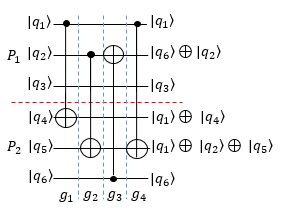
\includegraphics[width=50mm]{heuristic 1a}}
\subfigure {\label{b} 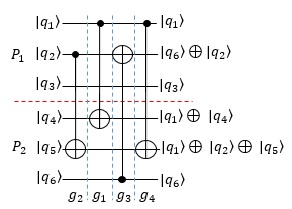
\includegraphics[width=50mm]{heuristic 1b}}
\subfigure {\label{c} 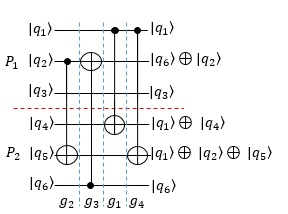
\includegraphics[width=50mm]{heuristic 1c}}
\caption{مثالی از هیوریستیک $I$}
\label{heuristicIe}
\end{figure}
\item
هیوریستیک $II$:
در روش دوم، ستون $i$ از ماتریس همجواری با ستون‌های مجاور خود $i+1 $ و $i+2 $ مقایسه می‌گردد. دو ستون کنار هم دارای یکی از سه حالت زیر هستند:
\begin{itemize}
\item
حالت ترکیب \footnote{\lr{Composition state}}: چنانچه در دوستون مجاور در سطر $i$ دو عنصر غیر صفر وجود داشته باشد، به اين معنا که این دو دروازه در کیوبیت شماره‌ی $q_i$ مشترک بوده و این دو ستون می‌توانند با یکدیگر ترکیب شوند. 
%\begin{equation}
%\text{if} \quad C[i][j]==C[i][j+1] \Rightarrow C[i][j]=max(C[i][j],C[i][j+1]) \& \quad \text{remove column j+1}
%\end{equation}
\item
حالت بلاک\footnote{\lr{Block state}}: چنانچه دو ستون پشت سرهم از ماتريس $C$ در سطر $i$ ام دارای دو عنصر غیر صفر با برچسب‌های متفاوت باشند، این دو ستون با یکدیگر ترکیب شده و مقدار برچسب ستون جدید به حالت $B$ تغییر مقدار می‌دهد. این وضعیت به آن معنی است که دو دروازه‌ی \lr{CNOT} پشت سرهم در یک کیوبیت مشترک بوده و برچسب آن‌ها متفاوت است. به‌عبارتی کیوبیت کنترلی یکی از دروازه‌ها کیوبیت هدف دیگری و یا بالعکس می‌باشد.
\item

حالت جابجاپذیر\footnote{\lr{Commutativity state}}: چنانچه دو ستون پشت سرهم در ماتریس در هیچ سطری دارای مقداری همزمان غیر صفر نباشند، این دو ستون می توانند با یکدیگر جابجا شوند. به عبارتی در هیج کیوبیت با یکدیگر اشتراک نداشته و از یکدیگر مستقل می‌باشند.
\end{itemize}
در شکل \ref{threestate} هر سه حالت ترکیب، بلاک و جابجا پذیر نشان داده شده است. الگوریتم 5 چگونگی اجرای هیوریستیک $II$ را در جهت کاهش تعداد دورنوردی‌های کوانتومی نشان می‌دهد. در این الگوریتم یکبار به از سمت چپ ماتریس $C$ شروع به پردازش نموده و رو به جلو حرکت می‌کنیم. پس از آن از انتهای ماتریس $C$ شروع نموده و در جهت رو به عقب حرکت نموده و عملیات را تکرار می‌کنیم. اين عمليات تا زماني ادامه مي‌يابد كه ابعاد ماتريس $C$ كاهش پيدا نكند.

 \begin{figure}
\centering     
\subfigure[حالت ترکیب]{\label{state1}\includegraphics[width=30mm]{composition}}
\subfigure[حالت بلاک]{\label{state2}\includegraphics[width=30mm]{block}}
\subfigure[حالت جابجاپذیر]{\label{state3}\includegraphics[width=30mm]{commu}}
\caption{سه حالت بیان شده}
\label{threestate}
\end{figure}






\begin{latin}
\begin{algorithm}
{
\fontsize{9}{1}
\caption{Heuristic II}
\begin{algorithmic}[1]
\Function {Heuristic II} {Matrix C}
\State\textcolor[rgb]{0.00,0.50,1.00}{ $\triangleright$ Input: Matrix C}
\State\textcolor[rgb]{0.00,0.50,1.00}{ $\triangleright$ Output: Optimized Connectivity Matrix}
\State $Plength\leftarrow 1$;
\State $Tlength\leftarrow 0;$

\While {$C.length< PCM.length$ }
\State $PCM\leftarrow C;$
\For{ $i=0 : TCM.length()$}
 \If {$C_{i}$  and $C_{i+1}$  in Composition Status}
  \State{$C_{i}$=Composition($C_{i},C_{i+1};$)}
 \EndIf
  \If {$C_i$  and $C_{i+1}  in Block Status$}
  \State{$C_{i}$=Block($C_{i},C_{i+1};$)}
 \EndIf
 \If {$C[i]$  and $C[i+1]$  in commute Status}
  \State{$TCM\leftarrow C;$}
  \State {$swap(C_i,C_{i+1});$}
  \If{$C_i$ and $C_{i+1}$ Not in composition or Block state}
      \State{$C\leftarrow TCM;$}
  \EndIf
 \EndIf
\EndFor
\For{i=C.length()-1: 1}
 \If {$C_{i}$  and $C_{i-1}$  in Composition Status}
  \State{$C_{i-1}$=Composition($C_{i},C_{i-1}$);}
 \EndIf
  \If {$C_i$  and $C_{i-1}$  in Block Status}
  \State{$C_{i-1}$=Block($C_{i},C_{i-1});$}
 \EndIf
 \If {$C_i$  and $C_{i-1}$  in commute Status}
  \State{$TCM\leftarrow C;$}
  \State {$swap(C_i,C_{i-1});$}
  \If{$C_i$ and $C_{i-1}$ Not in composition or Block state}
      \State{$C\leftarrow TCM;$}
  \EndIf
 \EndIf
\EndFor
\EndWhile
\State{$N_t\leftarrow teleportationnum(C)$}
\State {Return $N_t$;}
\EndFunction
\end{algorithmic}
}
\end{algorithm}
\end{latin}
\end{itemize}
\subsection{ بهینه‌سازی سطح دوم جهت كاهش دورنوردي‌ها در چند زیر سیستم}

\begin{latin}
\begin{algorithm}
{
\fontsize{9}{1}
\caption{Main algorithm}
\begin{algorithmic}[1]
\Function{Main algorithm} {Matrix C, Array P}
\State\textcolor[rgb]{0.00,0.50,1.00}{ $\triangleright$ Input: Matrix C, Array P}
\State\textcolor[rgb]{0.00,0.50,1.00}{ $\triangleright$ Output:Number of teleportations}
\State {$run$=\{0\};}
\State $teleportation\_cost\leftarrow 0;$
\For {$s=1:s\leq N_{g} $ }
\If {$g_{s}$ \textrm{is a single qubit or local two-qubit gate}}
\State {$run[s]=1;$}
\Else
\If {$run[s]== 0$} \State\textcolor[rgb]{0.00,0.50,1.00}{ $\triangleright$ $g_{s}$ is a non-local gate}
\State {$run[s]==1;$}
\State $teleportation\_cost\leftarrow teleportation\_cost+1;$
\State{[$index_{1,s},index_{2,s}]=Find\_qubits(g_s);$}
\State{$q\_teleport \leftarrow index_{1,s};$}
\State{$P_{q\_teleport}\leftarrow P_{index_{2,s}};$}
\State{ $g_{d} \leftarrow$ \textrm{Find the first gate applied on Qubit q\_teleport and another qubit be located in} $P_{q\_teleport };$}
\State {$run[d]=Eexecute(g\_s,g\_d,q\_teleport);$}
\EndIf
\EndIf
\EndFor
\EndFunction
\end{algorithmic}
}
\end{algorithm}
\end{latin}



در این الگوریتم آرایه‌ای به نام $run$ به اندازه تعداد دروازه‌های مدار در نظر گرفته شده است که مقدار $run[i]$ بیانگر حالت دروازه‌ی  $i$ می‌باشد که دارای مقدار 0 (در صورتی که دروازه $i$ام اجرا نشده باشد) و مقدار 1 ( در صورتی که دروازه‌ی $i$ام اجرا شده باشد) می‌باشد. دروازه‌ها یا همان ستون‌های ماتریس  $C$ از سمت چپ به راست با اندیس $s$ مورد بررسی قرار می گیرند. این دروازه در یکی از حالات زیر قرار دارد:
\begin{itemize}
\item
ستون $s$ از ماتریس $C$ بیانگر یک دروازه‌ی تک کیوبیتی است، در این صورت این دروازه اجرا شده و $run[i]=1 $ مقداردهی می‌گردد.
\item
ستون $s$ از ماتریس $C$ بیانگر یک دروازه‌ی محلی است، در این صورت این دروازه اجرا شده و $run[i]=1 $ مقداردهی می‌گردد.
\item
ستون $s$ بیانگر دروازه‌ی سراسری است و برای اجرا نیاز به یک دورنوردی کوانتومی دارد.
\end{itemize}
 در دو مورد اول دروازه $s$ بدون بررسی اجرا می‌گردد. اما در مورد سوم دروازه‌ی $s$ جهت اجرا نیاز به یک دورنوردی کوانتومی دارد. فرض شود دروازه‌ی $g_s=(index_{1,s},index_{2,s})$ دارای دو کیوبیت $index_{2,s}$ و $index_{1,s}$ بوده و یکی از کیوبیت‌های آن به نام $q\_teleport$ جهت اجرا به افراز مقصد دورنورد شود. در نتیجه $P_{q\_teleport}$ به شماره افرازی که $q\_teleport$ دورنوردی می‌شود، تغییر می‌یابد. سپس الگوریتم کل مدار را جستجو نموده تا دروازه ای اجرا نشده‌ای مانند $d$ را بیابد که برای اجرا شدن نیاز به $q\_teleport$ داشته باشد. فرض شود دروازه‌ی $g_{d} (index_{1,d},index_{2,d})$ اولین دروازه‌ی سراسری باشد که دارای یکی از شرایط زیر است:

\begin{itemize}
\item
یکی از کیوبیت‌های  $index_{1,d}$ یا  $index_{2,d}$ برابر با $q\_teleport$ باشد.
\item 
کیوبیت دیگر آن در $P_{q\_teleport}$ قرار گرفته باشد.
\end{itemize}

\begin {figure*}[h]
\begin{center}
\begin{tikzpicture}
\node at (0,0) (q1) {\ket{q_{1}}};
\node at (0,-1) (q2) {\ket{q_{2}}};
\node at (0,-2) (q3) {\ket{q_{3}}};
\node at (0,-3) (q4) {\ket{q_{4}}};
\node at (0,-4) (q5) {\ket{q_{5}}};
\node at (0,-5) (q6) {\ket{q_{6}}};

% Column 2
\node[control] (c20) at (2,0) {} ;edge [-] (q1);
\node[operator] (r25) at (2,-5) {} ;edge [-] (q6);
\draw[-] (c20) -- (2,-5.25);

\node[operator] (c50) at (5,0) {} ;edge [-] (q1);
\node[control] (r53) at (5,-3) {} ;edge [-] (q4);
\draw[-] (r53) -- (5,0.25);

\node[control] (c80) at (8,0) {} ;edge [-] (q1);
\node[operator] (r84) at (8,-4) {} ;edge [-] (q6);
\draw[-] (8,-4.25) -- (c80);

%gate
\node (end1) at (9,0) {} edge [-] (q1);\node (end2) at (9,-1) {} edge [-] (q2); \node (end3) at (9,-2) {} edge [-] (q3); \node (end4) at (9,-3) {} edge [-] (q4); \node (end4) at (9,-4) {} edge [-] (q5); \node (end4) at (9,-5) {} edge [-] (q6);
\node at (2,-6) {$g_{s}$}; \node at (5,-6) {$g_{k}$}; \node at (8,-6) {$g_{d}$};
%part
\draw [line1,dashed](-1,-3.5)-- (9.5,-3.5);\draw [line1,dashed](-1,-1.5)-- (9.5,-1.5);\draw [->] (c20) to [out=200, in=150,color=rgb] (r25); \node at (10,0) {$P_{1}$}; \node at (10,-2) {$P_{2}$}; \node at (10,-4) {$P_{3}$};\node at(2,0.5) {\small{Teleport $\ket{q_{1}}$ to $P_{3}$}};
\end{tikzpicture}
\end{center}
\caption{با دورنورد شدن $q_{1}$ به افراز $P_{3}$ دروازه‌ی $g_{d}$  مورد بررسی قرار می‌گیرد}
\label{figure4}
\end{figure*}
برای نمونه در مدار شکل \ref{figure4}، با دورنوردي شدن کیوبیت $q_1 $ از افراز $P_1 $ به افراز $P_3 $ اولین دروازه‌ی سراسری که در این کیوبیت با دروازه‌ی $g_s$ اشتراک دارد، دروازه‌ی $g_d$ می‌باشد. جهت بررسی اجرای این دروازه، تابعی بازگشتی به نام $Execute(g_{s},g_{d},q\_teleport)$ معرفی شده که اجرای دروازه‌ی $g_d$ را با دورنورد شدن $q\_teleport$ بررسی می‌کند. برای این تابع یکی از سه حالت زیر می‌تواند اتفاق بیفتد:
\begin{itemize}
\item
تعدادی دروازه‌ی اجرا نشده بین دروازه‌های $g_{s}$ و $g_{d}$ وجود داشته به‌طوری‌که این دروازه‌ها نتوانند قبل از اجرای $g_{d}$ اجرا شوند و اجرای دروازه‌ی $g_{d}$ به آن‌ها وابسته باشد. در این صورت این تابع مقداری  \lr{False} بر می‌گرداند.  فرض شود که در ماتریس $C$ ستون $k (s < k <d)$ بیانگر $g_{k} (index_{1,k},index_{2,k})$ اولین دروازه‌ی اجرا نشده و سراسری قبل از ستون $d$ باشد. بنابراین در ستون $k$ام از ماتریس دو سطر غیرصفر $index_{1,k}$ و  $index_{2,k}$ وجود دارد. این شرایط در معادله‌ی \ref{eq11} نشان داده شده است.
\begin{latin}
\begin{algorithm}
{
\fontsize{9}{1}
\caption{Execute (s, d, q\_teleport)}
\begin{algorithmic}[1]
\Function{Execute} {s,d,q\_teleport}
\State{$[index_{1,d},index_{2,d}]\leftarrow$ \textrm{Find two non-zero elements of C in Column} $d$}
\If {$s==d-1$}
\State {\Return 1;}
\EndIf
\State {$k\leftarrow d$}
\While {$s<k$}
\If {$run_{k}==1$}
\State {$k\leftarrow k-1$}
\State{$continue;$}
\EndIf
\If {\textrm{Gate $g_{k}$ is a non-local gate}}
\If {$C[index_{1,d},k]\ne 0 \| C[index_{2,d},k]\ne 0 $}
\If{\textrm{Common element of Columns $k$ and $d$ has Label 'C'}}
\State {$k\leftarrow k-1$}
\State{$continue;$}
\Else
%\State{$run[d]\leftarrow 0$}
\State {\Return 0;}
\EndIf
\Else
\State {$k\leftarrow k-1$}
\EndIf
\Else
\State {$break;$}
\EndIf
\EndWhile


\If{$k==s$}
\State {\Return 1;}
\EndIf

\State $r= Execute (g_{s},g_{k},q\_teleport)$;
\If {$r==1$}
\State { $run[k]=1;$}
\EndIf
\EndFunction
\end{algorithmic}
}
\end{algorithm}
\end{latin}

\begin{equation}\begin{split}
& index_{i,k} = index_{j,d} \quad \&\&\\
& P_{index_{\{1,2\} - i,k}} \ne P_{index_{\{1,2\}-j,d}} \quad \&\&\\
&\biggl( (C[k,index_{i,k}].label \ne C[d,index_{j,d}].label) \| \\
&C[k,index_{i,k}].label = C[d,index_{j,d}].label='t')\biggr) \\
&\exists i,j \in \{1,2\}\\
\end{split}
\label{eq11}
\end{equation}


\begin{figure}[htbp]
\centering     
\subfigure[]{\label{a}\begin{tikzpicture}
\node at (0,0) (q1) {\ket{q_{1}}};
\node at (0,-1) (q2) {\ket{q_{2}}};
\node at (0,-2) (q3) {\ket{q_{3}}};
\node at (0,-3) (q4) {\ket{q_{4}}};
\node at (0,-4) (q5) {\ket{q_{5}}};
\node at (0,-5) (q6) {\ket{q_{6}}};

% Column 2
\node[control] (c20) at (2,0) {} ;edge [-] (q1);
\node[operator] (r25) at (2,-5) {} ;edge [-] (q6);
\draw[-] (c20) -- (2,-5.3);

\node[control] (c50) at (5,0) {} ;edge [-] (q1);
\node[operator] (r53) at (5,-3) {} ;edge [-] (q4);
\draw[-] (5,-3.3) -- (c50);

\node[control] (c80) at (8,0) {} ;edge [-] (q1);
\node[operator] (r84) at (8,-4) {} ;edge [-] (q6);
\draw[-] (8,-4.3) -- (c80);

%gate
\node (end1) at (9,0) {} edge [-] (q1);\node (end2) at (9,-1) {} edge [-] (q2); \node (end3) at (9,-2) {} edge [-] (q3); \node (end4) at (9,-3) {} edge [-] (q4); \node (end4) at (9,-4) {} edge [-] (q5); \node (end4) at (9,-5) {} edge [-] (q6);
\node at (2,-6) {$g_{s}$}; \node at (5,-6) {$g_{k}$}; \node at (8,-6) {$g_{d}$};
%part
\draw [line1,dashed](-1,-3.5)-- (9.5,-3.5);\draw [line1,dashed](-1,-1.5)-- (9.5,-1.5);\draw [->] (c20) to [out=200, in=150,color=rgb] (r25); \node at (10,0) {$P_{1}$}; \node at (10,-2) {$P_{2}$}; \node at (10,-4) {$P_{3}$};\node at(2,0.5) {\small{Teleport $\ket{q_{1}}$ to $P_{3}$}};
\end{tikzpicture}
}
\medskip

\subfigure[]{\label{b}\begin{tikzpicture}
\node at (0,0) (q1) {\ket{q_{1}}};
\node at (0,-1) (q2) {\ket{q_{2}}};
\node at (0,-2) (q3) {\ket{q_{3}}};
\node at (0,-3) (q4) {\ket{q_{4}}};
\node at (0,-4) (q5) {\ket{q_{5}}};
\node at (0,-5) (q6) {\ket{q_{6}}};

% Column 2
\node[control] (c20) at (2,0) {} ;edge [-] (q1);\node[operator] (r25) at (2,-5) {} ;edge [-] (q6);\draw[-] (c20) -- (2,-5.25);
\node[operator] (c50) at (5,0) {} ;edge [-] (q1);\node[control] (r53) at (5,-3) {} ;edge [-] (q4);\draw[-] (r53) -- (5,0.25);
\node[control] (c80) at (8,0) {} ;edge [-] (q1);\node[operator] (r84) at (8,-4) {} ;edge [-] (q6);\draw[-] (8,-4.25) -- (c80);

%gate
\node (end1) at (9,0) {} edge [-] (q1);\node (end2) at (9,-1) {} edge [-] (q2); \node (end3) at (9,-2) {} edge [-] (q3); \node (end4) at (9,-3) {} edge [-] (q4); \node (end4) at (9,-4) {} edge [-] (q5); \node (end4) at (9,-5) {} edge [-] (q6);
\node at (2,-6) {$g_{s}$}; \node at (5,-6) {$g_{k}$}; \node at (8,-6) {$g_{d}$};
%part
\draw [line1,dashed](-1,-3.5)-- (9.5,-3.5);\draw [line1,dashed](-1,-1.5)-- (9.5,-1.5);\draw [->] (c20) to [out=200, in=150,color=rgb] (r25); \node at (10,0) {$P_{1}$}; \node at (10,-2) {$P_{2}$}; \node at (10,-4) {$P_{3}$};\node at(2,0.5) {\small{Teleport $\ket{q_{1}}$ to $P_{3}$}};
\end{tikzpicture}}
\end{figure}
\begin{figure}
\centering
\subfigure[]{\label{c}\begin{tikzpicture}
\node at (0,0) (q1) {\ket{q_{1}}};
\node at (0,-1) (q2) {\ket{q_{2}}};
\node at (0,-2) (q3) {\ket{q_{3}}};
\node at (0,-3) (q4) {\ket{q_{4}}};
\node at (0,-4) (q5) {\ket{q_{5}}};
\node at (0,-5) (q6) {\ket{q_{6}}};

% Column 2
\node[control] (c20) at (2,0) {} ;edge [-] (q1);\node[operator] (r25) at (2,-5) {} ;edge [-] (q6);\draw[-] (c20) -- (2,-5.3);
\node[control] (c52) at (5,-2) {} ;edge [-] (q1);\node[operator] (r54) at (5,-4) {} ;edge [-] (q4);\draw[-] (5,-4.3) -- (c52);
\node[control] (c80) at (8,0) {} ;edge [-] (q1);\node[operator] (r84) at (8,-4) {} ;edge [-] (q6);\draw[-] (8,-4.3) -- (c80);

%gate
\node (end1) at (9,0) {} edge [-] (q1);\node (end2) at (9,-1) {} edge [-] (q2); \node (end3) at (9,-2) {} edge [-] (q3); \node (end4) at (9,-3) {} edge [-] (q4); \node (end4) at (9,-4) {} edge [-] (q5); \node (end4) at (9,-5) {} edge [-] (q6);
\node at (2,-6) {$g_{s}$}; \node at (5,-6) {$g_{k}$}; \node at (8,-6) {$g_{d}$};
%part
\draw [line1,dashed](-1,-3.5)-- (9.5,-3.5);\draw [line1,dashed](-1,-1.5)-- (9.5,-1.5);\draw [->] (c20) to [out=200, in=150,color=rgb] (r25); \node at (10,0) {$P_{1}$}; \node at (10,-2) {$P_{2}$}; \node at (10,-4) {$P_{3}$};\node at(2,0.5) {\small{Teleport $\ket{q_{1}}$ to $P_{3}$}};
\end{tikzpicture}
}
\subfigure[]{\label{d}\begin{tikzpicture}
\node at (0,0) (q1) {\ket{q_{1}}};
\node at (0,-1) (q2) {\ket{q_{2}}};
\node at (0,-2) (q3) {\ket{q_{3}}};
\node at (0,-3) (q4) {\ket{q_{4}}};
\node at (0,-4) (q5) {\ket{q_{5}}};
\node at (0,-5) (q6) {\ket{q_{6}}};

% Column 2
\node[control] (c20) at (2,0) {} ;edge [-] (q1);\node[operator] (r25) at (2,-5) {} ;edge [-] (q6);\draw[-] (c20) -- (2,-5.3);
\node[operator] (c52) at (5,-2) {} ;edge [-] (q1);\node[control] (r54) at (5,-4) {} ;edge [-] (q4);\draw[-] (5,-1.75) -- (r54);
\node[control] (c80) at (8,0) {} ;edge [-] (q1);\node[operator] (r84) at (8,-4) {} ;edge [-] (q6);\draw[-] (8,-4.3) -- (c80);

%gate
\node (end1) at (9,0) {} edge [-] (q1);\node (end2) at (9,-1) {} edge [-] (q2); \node (end3) at (9,-2) {} edge [-] (q3); \node (end4) at (9,-3) {} edge [-] (q4); \node (end4) at (9,-4) {} edge [-] (q5); \node (end4) at (9,-5) {} edge [-] (q6);
\node at (2,-6) {$g_{s}$}; \node at (5,-6) {$g_{k}$}; \node at (8,-6) {$g_{d}$};
%part
\draw [line1,dashed](-1,-3.5)-- (9.5,-3.5);\draw [line1,dashed](-1,-1.5)-- (9.5,-1.5);\draw [->] (c20) to [out=200, in=150,color=rgb] (r25); \node at (10,0) {$P_{1}$}; \node at (10,-2) {$P_{2}$}; \node at (10,-4) {$P_{3}$};\node at(2,0.5) {\small{Teleport $\ket{q_{1}}$ to $P_{3}$}};
\end{tikzpicture}
}
\caption{مدار کوانتومی ارائه شده با پنج دروازه و چهار کیوبیت. در مدارات \ref{a} تا \ref{d}چهار حالتی که منجر به برگرداندن مقداری \lr{False} در مدار می‌شوند، نشان می‌دهد}
\end{figure} 

این معادله بیان می‌کند دروازه‌های $g_{k}$ و $g_{d}$ در یک کیوبیت با برچسب‌های متفاوت مشترک بوده و یا اینکه در کیوبیت مشترک دارای برچسب $'T'$ مي‌باشند. همچنین کیوبیت دیگر آن‌ها در دو افراز متفاوت قرار داشته باشد. در این صورت دروازه‌ی $g_{d}$ از لحاظ اجرایی وابسته به اجرای دروازه‌ی $g_{k}$ است. و از آنجایی که دروازه‌ی $g_{k}$ جهت اجرا نیاز به یک دورنوردی دارد، در نتیجه دروازه‌‌ی $g_{d}$ نمی‌تواند اجرا شود و این تابع مقداری \lr{False} برمی‌گرداند. مدارات \ref{a} تا \ref{d} دارای این شرایط می‌باشند. در این مدارات، کیوبیت $q_{1}$ از افراز $P_{1}$ به افراز $P_{3}$ دورنورد می‌گردد. در نتیجه اولین دروازه‌ی سراسری اجرا نشده که نیاز به این کیوبیت دارد، دروازه‌ی $g_{d}$ می‌باشد. این دروازه جهت اجرا نیازی به بررسی این دارد که آیا بین دروازه‌های $g_{d}$ و $g_{s}$ محدودیت‌های پیش نیازی برای دروازه‌ی $g_{d}$ رعایت شده است؟ پس از بازگشت به عقب اولین دروازه‌ی اجرا نشده‌ی سراسری مانند $g_{k}$ وجود دارد که اجرای $g_{d}$ به اجرای آن وابسته است. در نتیجه دروازه‌ی $g_{d}$ نمی‌تواند اجرا گردد و این تابع مقداری \lr{False} بر می‌گرداند.

چنان‌چه دروازه‌‌ی $g_{k}$ دروازه‌‌ای سراسری بوده که با دروازه‌ی $g_{d}$ دارای کیوبیت مشترک با برچسب $`c'$ باشد، آنگاه دروازه‌ی $g_d$ و $g_k$ از لحاظ اجرایی به یکدیگر وابستگی نداشته و بنابراین می‌توان از روی دروازه‌ی $g_k$ عبور نموده و اجرای آن را بررسی نکرد. این مفهوم در شکل \ref{e} نشان داده شده است. در این حالت دروازه‌های $g_d$ و $g_k$ در کیوبیت $q_5 $ با برچسب $'c'$ مشترک بوده است. در این حالت می‌توان عدم اجرای دروازه‌ی $g_k$ را در نظر نگرفته و سایر دروازه‌های ماقبل از آن را بررسی نمود. به عبارتی وجود دروازه‌ی اجرا نشده‌ی $g_k$ تاثیری روی اجرا نشدن دروازه‌ی $g_d$ نداشته و باعث توقف تابع  \lr{Execute} نمی‌گردد. در نتیجه سایر دروازه‌های ما قبل از این دروازه تا رسیدن به دروازه‌ی $g_s$ بررسی می‌گردد. این شرایط در معادله‌ی \ref{eq12} بیان شده است.
\begin{equation}
\begin{split}
&index_{i,k}= index_{j,d}\quad \&\& \\ 
&({C[ {k,inpu{t_{i,k}}} ].label =C[{d,inpu{t_{j,d}}} ].label = 'c'} ) \\
&\exists i,j \in\{1,2\}\\
\label{eq12}
\end{split}
\end{equation}

\begin{figure}
\centering
\subfigure[مشترک بودن دو دروازه‌ی $g_d$ و $g_k$ در کیوبیت $q_5$ با برچسب $'c'$]{\label{e}
\begin{tikzpicture}
\node at (0,0) (q1) {\ket{q_{1}}};
\node at (0,-1) (q2) {\ket{q_{2}}};
\node at (0,-2) (q3) {\ket{q_{3}}};
\node at (0,-3) (q4) {\ket{q_{4}}};
\node at (0,-4) (q5) {\ket{q_{5}}};
\node at (0,-5) (q6) {\ket{q_{6}}};

% Column 2
\node[control] (c20) at (2,0) {} ;edge [-] (q1);\node[operator] (r25) at (2,-5) {} ;edge [-] (q6);\draw[-] (c20) -- (2,-5.3);
\node[operator] (c52) at (5,-2) {} ;edge [-] (q1);\node[control] (r54) at (5,-4) {} ;edge [-] (q4);\draw[-] (5,-1.75) -- (r54);
\node[operator] (r80) at (8,0) {} ;edge [-] (q1);\node[control] (c84) at (8,-4) {} ;edge [-] (q6);\draw[-] (8,0.3) -- (c84);

%gate
\node (end1) at (9,0) {} edge [-] (q1);\node (end2) at (9,-1) {} edge [-] (q2); \node (end3) at (9,-2) {} edge [-] (q3); \node (end4) at (9,-3) {} edge [-] (q4); \node (end4) at (9,-4) {} edge [-] (q5); \node (end4) at (9,-5) {} edge [-] (q6);
\node at (2,-6) {$g_{s}$}; \node at (5,-6) {$g_{k}$}; \node at (8,-6) {$g_{d}$};
%part
\draw [line1,dashed](-1,-3.5)-- (9.5,-3.5);\draw [line1,dashed](-1,-1.5)-- (9.5,-1.5);\draw [->] (c20) to [out=200, in=150,color=rgb] (r25); \node at (10,0) {$P_{1}$}; \node at (10,-2) {$P_{2}$}; \node at (10,-4) {$P_{3}$};\node at(2,0.5) {\small{Teleport $\ket{q_{1}}$ to $P_{3}$}};
\end{tikzpicture}
}
\end{figure}


%%%%%%%%%%%%%%%%%%%%5circuit
\item
در این حالت تابع $Execute$ دروازه‌ای با شرایط بیان شده در معادله‌ی \ref{eq14} در مدار یافت می‌نماید. چنانچه دروازه‌ی $g_k$ یک دروازه‌ی اجرا نشده‌ی تک کیوبیتی و یا دروازه‌ای محلی باشد که در یک کیوبیت با دروازه‌ی $g_d$ اشتراک داشته باشد، آنگاه این تابع به صورت بازگشتی اجرای دروازه‌ی $g_k$ را بررسی می‌نماید و به‌صورت $Execute(g_s,g_k, q_{teleport})$  فراخوانی می‌گردد.
\begin{figure}[htbp]
\centering
\subfigure[دروازه‌ی $g_k$ دروازه‌ای محلی و دو کیوبیتی بوده که اجرای دروازه‌ی $g_d$ به آن وابسته است]{\label{f}\begin{tikzpicture}
\node at (0,0) (q1) {\ket{q_{1}}};
\node at (0,-1) (q2) {\ket{q_{2}}};
\node at (0,-2) (q3) {\ket{q_{3}}};
\node at (0,-3) (q4) {\ket{q_{4}}};
\node at (0,-4) (q5) {\ket{q_{5}}};
\node at (0,-5) (q6) {\ket{q_{6}}};

% Column 2
\node[control] (c20) at (2,0) {} ;edge [-] (q1);\node[operator] (r25) at (2,-5) {} ;edge [-] (q6);\draw[-] (c20) -- (2,-5.3);
\node[control] (c55) at (5,-5) {} ;edge [-] (q1);\node[operator] (r54) at (5,-4) {} ;edge [-] (q4);\draw[-] (5,-3.7) -- (c55);
\node[operator] (r80) at (8,0) {} ;edge [-] (q1);\node[control] (c84) at (8,-4) {} ;edge [-] (q6);\draw[-] (8,0.3) -- (c84);

%gate
\node (end1) at (9,0) {} edge [-] (q1);\node (end2) at (9,-1) {} edge [-] (q2); \node (end3) at (9,-2) {} edge [-] (q3); \node (end4) at (9,-3) {} edge [-] (q4); \node (end4) at (9,-4) {} edge [-] (q5); \node (end4) at (9,-5) {} edge [-] (q6);
\node at (2,-6) {$g_{s}$}; \node at (5,-6) {$g_{k}$}; \node at (8,-6) {$g_{d}$};
%part
\draw [line1,dashed](-1,-3.5)-- (9.5,-3.5);\draw [line1,dashed](-1,-1.5)-- (9.5,-1.5);\draw [->] (c20) to [out=200, in=150,color=rgb] (r25); \node at (10,0) {$P_{1}$}; \node at (10,-2) {$P_{2}$}; \node at (10,-4) {$P_{3}$};\node at(2,0.5) {\small{Teleport $\ket{q_{1}}$ to $P_{3}$}};
\end{tikzpicture}
}
\subfigure[دروازه‌ی $g_k$ دروازه‌ای تک کیوبیتی بوده که اجرای دروازه‌ی $g_d$ به آن وابسته است.]{\label{h}\begin{tikzpicture}
\node at (0,0) (q1) {\ket{q_{1}}};
\node at (0,-1) (q2) {\ket{q_{2}}};
\node at (0,-2) (q3) {\ket{q_{3}}};
\node at (0,-3) (q4) {\ket{q_{4}}};
\node at (0,-4) (q5) {\ket{q_{5}}};
\node at (0,-5) (q6) {\ket{q_{6}}};

% Column 2
\node[control] (c20) at (2,0) {} ;edge [-] (q1);\node[operator] (r25) at (2,-5) {} ;edge [-] (q6);\draw[-] (c20) -- (2,-5.3);
\node[hadamard] (h) at (5,-4) {H} ;
\node[operator] (r80) at (8,0) {} ;edge [-] (q1);\node[control] (c84) at (8,-4) {} ;edge [-] (q6);\draw[-] (8,0.3) -- (c84);

%gate
\node (end1) at (9,0) {} edge [-] (q1);\node (end2) at (9,-1) {} edge [-] (q2); \node (end3) at (9,-2) {} edge [-] (q3); \node (end4) at (9,-3) {} edge [-] (q4); \node (end4) at (9,-4) {} edge [-] (q5); \node (end4) at (9,-5) {} edge [-] (q6);
\node at (2,-6) {$g_{s}$}; \node at (5,-6) {$g_{k}$}; \node at (8,-6) {$g_{d}$};
%part
\draw [line1,dashed](-1,-3.5)-- (9.5,-3.5);\draw [line1,dashed](-1,-1.5)-- (9.5,-1.5);\draw [->] (c20) to [out=200, in=150,color=rgb] (r25); \node at (10,0) {$P_{1}$}; \node at (10,-2) {$P_{2}$}; \node at (10,-4) {$P_{3}$};\node at(2,0.5) {\small{Teleport $\ket{q_{1}}$ to $P_{3}$}};
\end{tikzpicture}
}

\end{figure}
\item

چنانچه هیچ درواز‌ای مانند $g_k$ با شرایط بیان شده در دو حالت قبل بین دروازه‌های $g_s$ و $g_d$ پیدا نگردید، در نتیجه می‌توان با دورنوردی نمودن کیوبیت $q\_{teleport}$ علاوه بر اجرای دروازه‌ی $g_s$ دروازه‌ی $g_d$ نیز اجرا گردد. در نتیجه $run[d]=1$ مقداردهي شده و تابع مقداری \lr{True} بر می‌گرداند.
\end{itemize}

\section{خلاصه}
در این فصل راه کار پیشنهادی برای توزیع مدار کوانتومی در چند زیر سیستم با رویکرد کاهش تعداد دورنوردی‌های کوانتومی و توزیع متوازن کیوبیت‌ها ارائه شد. به دلیل پیچیدگی بالای سیستم‌های کوانتومی، کاهش تعداد دورنوردی‌ها در یک سطح امری دشوار بود. جهت حل این مشکل، بهینه سازی دو سطحی در نظر گرفته شد. در سطح اول سعی گردید تا بتوان کیوبیت‌های مدار در تعدادی زیر سیستم به طور متوازن توزیع گردد به طوری که تعداد ارتباطات لازم یا همان تعداد دروازه‌های سراسری بین زیر سیستم‌ها کاهش یابد. زمانی که یک کیوبیت از یک دروازه‌ی محلی از مبدا خود به مقصد مورد نظر دورنوردی می‌گردد، می‌تواند توسط سایر دروازه‌ها بدون برگشت آن به مقصد خود مورد استفاده قرار گیرد. این امر کاهش چشمگیری در کاهش تعداد دورنوردی‌های مورد نیاز دارد. با در نظر گرفتن این ایده در سطح دوم، می‌توان تعداد دورنوردی‌ها را کاهش داد.

در ابتدا یک مدل ریاضی با استفاده از برنامه ریزی خطی جهت افرازبندی مدار کوانتومی ارائه شد که در آن دو هدف مورد نظر در نظر گرفته شد. سپس الگوریتم‌های افرازبندی کیوبیت‌ها در دو زیر سیستم و چند زیر سیستم کوانتومی در سطح اول شد. سپس در سطح دوم به ارائه تعدادی هیوریستیک جهت بهینه‌سازی سطح دوم پرداخته شد.